\documentclass[parskip=full]{scrartcl}
\usepackage[utf8]{inputenc} % use utf8 file encoding for TeX sources
\usepackage[T1]{fontenc}    % avoid garbled Unicode text in pdf
\usepackage[english]{babel}  % english hyphenation, quotes, etc
\usepackage[colorlinks=true,linkcolor=blue]{hyperref}       % detailed hyperlink/pdf configuration
\usepackage{graphicx}       % provides commands for including figures
\usepackage{csquotes}       % provides \enquote{} macro for "quotes"
\usepackage{enumitem}
\usepackage{multicol}
\usepackage{underscore}
\setlength{\columnsep}{4cm}
%\usepackage{lscape}	% provides landscape portrait

\usepackage{pdflscape}	% provides horizental landscape portrait


\usepackage{pdfpages}	% add another pdf in  Latex

\usepackage{tikz}


\usepackage{verbatim}	% provides multi-line comments

\usepackage{afterpage}
\usepackage{ragged2e}
\usepackage[export]{adjustbox}
\newcommand\tab[1][1cm]{\hspace*{#1}}


\title{\Huge \textbf{HePICS Test-Phase Document}}
\date{\today \vspace{+10ex}}
\author{Andres Stober \\
	\and Mehyar Cherni \\
	\and Ibrahim Bouriga \\ 
	\and Linjuan Fan \\
	\and Bahaa Mahjane \\ }

\begin{document}

\maketitle
\thispagestyle{empty}

\begin{tikzpicture}[remember picture, overlay]
  \node [anchor=north west, inner sep=0.5pt, yshift=-20pt,xshift=20pt]  at (current page.north west)
     {
\includegraphics[height=1.9cm]{Logo_KIT}};
\end{tikzpicture}

\begin{figure}[b]
\centering
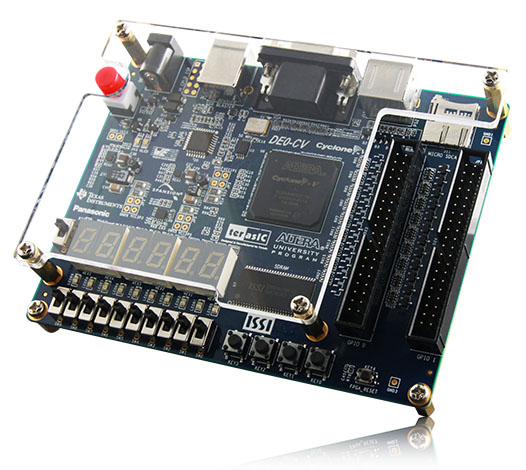
\includegraphics[width=0.45\textwidth, center]{boardimage.jpg}
\end{figure}

\pagebreak

\tableofcontents
\thispagestyle{empty}
\pagebreak

\section{Test Tools}

    \subsection{Google Test}
    \tab Google Test is a unit testing library for the C++ programming language, based on the xUnit architecture. This section describes some good reasons why we decided to use this framework.
    
    \begin{itemize}
        \item is designed to be portable and it works around various bugs in various compilers and environments
        \item its framework has built-in assertions that are deployable in software where exception handling is disabled
        \item runs the tests is simple and it’s easy to write assertions that generate informative messages
        \item automatically detects your tests and doesn’t require you to enumerate them in order to run them
        \item its framework provides excellent support for handling such situations. You can repeat the same test a lot of times using the Google framework
    \end{itemize}
    
    \subsection{gcov - Coverage Testing Tool}
    \tab gcov is a test coverage program. We used it in concert with GCC to analyze our programs to help create more efficient, faster running code and to discover untested parts of your program. We used gcov as a profiling tool to help discover where our optimization efforts will best affect our code.
    
    \tab gcov profiling tools helped us analyze our code's performance. By using gcov we found some basic performance statistics, such as:
    \begin{itemize}
        \item how often each line of code executes
        \item what lines of code are actually executed
        \item how much computing time each section of code uses
    \end{itemize}
    

\section{Layer Tests}

   \subsection {Fully Connected Layer Tests}
   \tab This layer basically takes an input volume (whatever the output is of the conv or ReLU or pool layer preceding it) and outputs an N dimensional vector where N is the number of classes that the program has to choose from.
   
   \tab TEST(fully_connected_layer, test_fully_connected_layer): for this test we have created this objects:
   \begin{itemize}
       \item weights: object of an Image
       \item fully_connected_layer: object of Fully Connected Layer class
       \item inputImage: input image
       \item expectedOutput: expected output
       \item outputFrom_Fully_connected_layer: output of the fully connected layer for the input image
   \end{itemize}
   
   \tab after creating this objects and adding the data to each object we tested if the expected output is equals to the output of the connected layer with \textbf{ASSERT_EQ}

   \subsection{Maxpooling Layer Tests}
   \tab This layer is to progressively reduce the spatial size of the representation to reduce the amount of parameters and computation in the network, and hence to also control overfitting. 
   
   \tab TEST(max_pool_layer, test_max_pool):
   for this test we have created this object:
   
   \begin{itemize}
       \item mxp: object of max pooling layer
       \item input:input image in size 3x3x2x1
       \item expectedOutput: expected output 
       \item newOutput:output after applying forward_layer method
   \end{itemize}

   \tab TEST(max_pool_layer2, test_max_pool2):
   for this test we have created this object:
   
   \begin{itemize}
       \item input2: input image in size 6x6x2x1
       \item expectedOutput2: expected output 
       \item newOutput2:output after applying forward_layer method
   \end{itemize}
   

   \tab For each of these tests we created an input image, an expected output and an object of max pool layer. After adding the data for each object we tested with \textbf{ASSERT_EQ} if the output of the max pool layer as we expect it in the output that we created. 
   
   \subsection{Local Response Normalization Layer Tests}
   
   \tab The local response normalization layer performs a kind of “lateral inhibition” by normalizing over local input regions. In ACROSS_CHANNELS mode, the local regions extend across nearby channels, but have no spatial extent.
   
   \tab TEST(local_response_normalization_layer, test_local_response_normalization_layer): for this test we have created this object:
   
   \begin{itemize}
       \item lrn: object of local response normalization layer
       \item input: input image in size 2x2x2x1
       \item expectedOutput:expected output
       \item output: output after applying forward_layer method 
   \end{itemize}
   
   \tab after creating this objects and adding the data to each object we tested if the expected output is equals to the output of the lrn layer with \textbf{ASSERT_EQ}.
   
   

\end{document}
